\documentclass[12pt]{report}
\usepackage{WUthesis}
%\usepackage[latin1]{inputenc}
\usepackage{amsmath}
\usepackage{gensymb}
\usepackage{amsfonts}
\usepackage{amssymb} 
\usepackage{siunitx}
\usepackage{graphicx}
\usepackage{color, colortbl}
\graphicspath{ {images/} }
%\usepackage{listings}
%\usepackage{minted}
%\usepackage[revision]{revann}
\usepackage{tikz}
\usepackage{array}
\usepackage{subcaption}
\usepackage{caption}
\usepackage{soul}
\usepackage{physics}
\usepackage{booktabs}
%\usepackage[per-mode=symbol]{siunitx}
\sisetup{group-separator={,}, per-mode=symbol}

\usepackage[style=numeric, url=false, isbn=false, backend=bibtex]{biblatex}
\addbibresource{thesis_bib.bib}

\newcommand{\comment}[1]{{\footnote{\color{green!40!black}#1}}}
\newcommand{\inlinecomment}[1]{{\bf\color{green!40!black} [\scriptsize #1]}}
\newcommand*\circled[1]{%
  \tikz[baseline=(char.base)]\node[shape=circle,fill=green!60!black!20!white, draw=green!40!black,,text=black,inner sep=0.2pt,font=\tiny\bf,minimum size=8pt] (char) {#1};}
\renewcommand\thefootnote{\protect\circled{\arabic{footnote}}}



\begin{document}


\title{An Analysis of Fireballs from Willamette's D6 AllSky Survey}
\author{Peter Joseph Gibson}
\thesissupervisor{Dr. Jed Rembold}

\maketitle


\newpage

\begin{center}
\textbf{Presentations and publications}

P. Gibson, Analyzing Fireballs from Willamette's D6 AllSky Survey, Poster Presentation at Willamette University, Research Seminar II: Thesis Presentation (May 2019)
\bigskip


P. Gibson, Analyzing Fireballs from Willamette's D6 AllSky Survey, Oral Presentation at Willamette University, Research Seminar II: Thesis Presentation (April 2019)
\bigskip

P. Gibson, Analyzing Fireballs from Willamette's D6 AllSky Survey, Oral Presentation at Willamette University, Research Seminar I: Status Report Presentation (December 2018)
\bigskip

P. Gibson, Analyzing Fireballs from Willamette's D6 AllSky Survey, Oral Presentation at Willamette University, Advanced Techniques in Experimental Physics: Senior Proposal Presentation (April 2018)

\end{center}



\begin{acknowledgments}
I would like to thank the following professors for their tremendous support and advice throughout my Willamette experience:
\begin{itemize}
    \item Dr.~Jed Rembold for teasing me and providing me with Hershey's Kisses as a consolation for his hate.
    \item Dr.~Rick Watkins for telling me "You got this!" in trying times.
    \item Dr.~Daniel Borrero, Dr.~Michaela Kleinart, Dr.~David Altman for their kindness and unwavering confidence in our graduating class.
\end{itemize}

I would also so like to thank the following people for helping me through countless homework problems, talking down my problems, and also picking on me when I deserve it:

\begin{itemize}
    \item Trent Jones for being a below par friend and an above par golfer.
    \item Jo Stensass for serving me all sorts of help along the way and providing a willingness to set me up for success.
    \item The wizards who answer questions on Stack Overflow and spend time editing Wikipedia to make it a more reliable resource.
    \item Not only to God but to Jesus.
\end{itemize}

Lastly, but perhaps most importantly, I would like to thank my mother and father for their unconditional love and for providing me with countless wonderful life opportunities such as the entirety of my college experience.  There is no argument that I would not be at this point without them.

\end{acknowledgments}

\begin{abstract}
\begin{flushleft}

\textbf{\textsc{\LARGE General Abstract}}

\vspace{0.2 in}

As fireballs, more commonly known as shooting stars, fly through Earth’s atmosphere at breakneck speeds, they emit light that can be observed from our planet’s surface. 
Willamette’s D6 AllSky Survey is a camera system that probes the night sky for these events.
One method of quantifying the number of events seen is through what is called the flux.
Flux describes the number of events that occur per unit time per unit area.
Because one camera system can only observe $<0.4\%$ of Earth’s total sky area, amateur astronomers hold a significant role in fireball observations.
Their observations provide a robust data sample size that can then be used to gain a deeper understanding of the flux rates and property distributions of fireballs.
While complex multi-camera professional systems currently exist, there is need for more economic, accessible, and versatile systems. 
We will discuss the feasibility of our current observational setup and how it compares to more elaborate existing systems.
\vspace{0.25 in}

\textbf{\textsc{\LARGE Technical Abstract}}

\vspace{0.2 in}

Fireballs, more technically known as bolides, are recognizable by the light they emit through ablation in the atmosphere.. 
The D6 AllSky Camera was designed by Dr.~Jed Rembold and Kyle McSwain as an alternative observation system for fireball research. 
It is smaller, cheaper, and much more portable, than most existing systems used by professional astronomers. 
By measuring and comparing distributions and the average flux of fireballs to other observation networks, we aim to assess the feasibility and efficiency of using the D6 AllSky Camera for fireball research.  
Due to poor weather and other complications, our observed data sample this year was not sufficiently large to produce a reliable average flux rate.
However the versatile framework and software pipeline established in this research will assuredly aid in the analysis of fireballs throughout further observations with the D6 AllSky Camera.

\end{flushleft}

\end{abstract}

\tableofcontents
%\listoftables
\listoffigures

\chapter{Introduction}

Based on a rough estimate, there are about \num{10000} trillion ants, \num{7.6} billion humans, and a few million elephants in the world.
When considering this data set, one might come to the conclusion that there are more small objects in the world than there are large objects.
It so happens that this conclusion not only holds true on Earth, but it also holds true in our universe.
For every singular large object in space, there are significantly more smaller objects.
To provide a parallel to the animal example, in our solar system, there is one star, eight planets, and an almost incomprehensible number of small rocks traveling through space. 

In space, distances manifest on an extremely large scale when compared to on-Earth distances.  
Similarly, objects in space travel significantly faster than objects observed on Earth.
For example, the Earth travels at approximately \SI{30}{\kilo\meter\per\second} while small rocks can travel between \SIrange{11}{70}{\kilo\meter\per\second}.  
The speeds of these rocks exceed the muzzle velocity of a bullet \cite{russell_photometry_2018}.
When we observe a meteor shower, we are witnessing a barrage of these bullet-like rocks.  
Fortunately for mankind, Earth’s atmosphere provides a protective shield.
This shield is composed of tightly packed (relative to the vacuum of space) air molecules.

As a rocky object travels through Earth’s atmosphere, it collides with particles and burns in a phenomena known as ablation.  
The result is a release of energy in the form of both heat and light.  
The objects which ignite and begin to break down are called meteors.
As a meteor releases light, the brightness can be measured from Earth's surface and is expressed as a photometric (visual) magnitude. 
The brightest meteors, which have a magnitude less than $-4$, are referred to as fireballs.
By observing the magnitude, duration, and other properties of individual fireball events, an observer can estimate the energies and sizes of these near-Earth rocky objects.

\begin{figure}[ht!]
  \centering
  \includegraphics[scale=0.9]{images/flux_brown.png}
  \caption[A plot of bolide flux vs. energy and diameter using a wide collection of data.]{A plot of bolide flux vs. energy and diameter using a wide collection of data.  The two $x-$axes represent physical characteristics of fireballs while the $y-$axis represent various flux rates.  We see that larger and more energetic events are far less likely than their less powerful counterparts.  We hope to eventually compare our flux rates to low-energy collision flux rates depicted in this plot.}
  \label{brown}
\end{figure}

Studying these near-Earth objects can give us good estimates for how many objects we might expect to see pass through a given area of space within a specific amount of time.
This measurement is called flux.
By determining flux, we can more accurately predict the likelihood of objects in space being hit by near-Earth objects. 
Although the case may have been an extreme one, the space satellite Olympus was struck and destroyed by a meteoroid during the Perseid meteor shower in 1993 \cite{bobrowsky_comet/asteroid_nodate}.
An accurate flux estimate would allow us to estimate the probability that a fireball of a given mass would collide with Earth.
These estimates, similarly to predictions surrounding volcanic or earthquake activity, give us insight into past events and help us foresee likelihoods of future events.

This project aims to analyze the feasibility of the Willamette D6 AllSky Camera, a new alternative camera system for conducting fireball research. 
Occupying about the same space as a traffic cone, this camera is easily transportable.
Contrasting many existing systems that run using powerful computers, our camera is operated by a microcontroller.
To determine the feasibility of our setup, we will compare our measured flux rates to those found by more well-established systems.
Peter Brown, an astronomy researcher, created a now-famous relationship between flux and bolide energy/diameter \cite{brown_p_flux_2002}.
As seen in Figure~\ref{brown}, bolides with extremely high energies are far less likely to collide with earth than their less energetic counterparts.
By comparing our flux rates to those found in Figure~\ref{brown} (for small energies), we can assess how consistent our data is with existing professional systems.

This paper is broken up into several sections for ease of reading. Chapter 2 details useful information surrounding fireballs, their importance, existing research, and the theory necessary to calculate flux rates. 
The remaining chapters focus on our methods, data, and final conclusions.   

\chapter{Background}

Thanks to a dense protective atmosphere, Earth can withstand impacts from dust to boulder-sized objects traveling faster than bullets without so much as a dent on Earth's surface.
Many of these near-Earth objects are extremely small and don't leave much of a trace, but larger objects can leave a trail of light visible from Earth's surface as they burn up in our atmosphere.
In this chapter, we will discuss the classification of near-Earth objects, how fireballs are observed, and give important insight as to why and how we will compare our photometric survey with others.


\section{Description of Fireballs}

When considering types of near-Earth objects, many names come to mind: asteroids, meteors, meteorites, and fireballs are all often used interchangeably. 
However, there are several key distinctions between these objects.  
Traveling through space, asteroids are the largest of this group and are generally over \SI{10}{\meter} in diameter \cite{steel_meteoroid_1996}. 
These objects are responsible for massive craters that are visibly present on the Moon.
Meteoroids are anywhere between \SI{10}{\micro\meter} and \SI{10}{\meter} and are far more numerous than their asteroid cousins.  

Meteoroids or asteroids that pass through Earth's atmosphere become meteors.
As a meteor passes through our atmosphere, it begins to ablate.
Ablation begins when a fast moving meteor, typically traveling over \SI{10}{\meter/\second}, encounters air particles that slow it down.
This loss of kinetic energy is turned into heat and is hot enough to vaporize outer layers of the meteor.  
Atoms within these vaporized outer layers and nearby air molecules get energetically excited and then release light as they relax back to their natural state.
The amount of light that reaches an observer on Earth's surface can be measured in terms of apparent magnitude.
Magnitude is represented on an inverse $\log_{10}$ scale where dimmer objects are represented by high numbers and brighter objects are lower, and in many cases negative, values.
Magnitude is calculated as:

\begin{equation}
m = -2.5 \log_{10}(I/I_0)
\label{magnitude_equation}
\end{equation}

 
where $I$ is the intensity of the meteor/fireball and $I_0$ is the intensity of a reference brightness.  
Both intensity measurements are in units of $\si{\watt/\meter^2}$.
Meteors with an apparent magnitude below $-4$ qualify as bolides or fireballs.
For reference, in its brightest phase, Venus is a magnitude $-4.4$ planet while the dimmer Jupiter has a magnitude of $-2.1$ \cite{rao_venus_nodate}.
If an object is massive enough to withstand the heat of ablation in Earth's atmosphere and make it to the surface of Earth, it is classified as a meteorite. 
These are rare, occurring less than $200$ times per year.
Because meteorites are essentially rock remnants, they provide valuable information about the initial asteroid's origins.
While there is some overlap between asteroids, meteoroids, meteors, fireballs, and meteorites, their definitions are important to distinguish.
Figure~\ref{jed} graphically summarizes the relationship between these 5 terms.

\begin{figure}[ht!]
  \centering
  \includegraphics[scale=0.3]{images/jed_zoomedin.png}
  \caption[A depiction of near-Earth object classification.]{A depiction of near-Earth object classification.  Asteroids and meteoroids may be found in space, while meteors and their brighter counterparts, fireballs, burn up through Earth's atmosphere.  Unlike ordinary fireballs, meteorites remain intact and strike the surface of the Earth.}
  \label{jed}
\end{figure}

Our project specifically focuses on fireballs.
A fireball passing through the sky is referred to as a fireball event.
We may further classify fireball events into two categories: sporadic events and meteor shower events.
Meteor showers share an important relationship with comets.
Comets are celestial objects much larger than asteroids.
As comets travel through space, small bits of rock and ice separate from them.
This process is due to differences in pressures and heat on different areas of the comet.
Comet fragments make up a majority of the substance in meteor showers.


Meteor showers occur when Earth's orbit crosses paths with the orbit of a collection of debris. 
Such collections often orbit large masses such as Jupiter or the sun \cite{trigo-rodriguez_2006_2007}.
For example, the Perseid meteor shower has a highly elliptical orbit around the sun as seen in Figure~\ref{perceid}.  

\begin{figure}[ht!]
  \centering
  \includegraphics[scale=1.4]{images/persiod_shower.jpg}
  \caption[The Perseid meteor shower and its relation to our solar system.]{The Perseid meteor shower and its relation to our solar system.  Earth's orbit is shown in red (just inside of the yellow ring) while meteors in the shower are depicted as white dots.}
  \label{perceid}
\end{figure}

In contrast, there is debris in space that is not connected to any meteor shower. 
Events stemming from random debris are called sporadic events.
Debris in space can collect and becomes part of a larger system such as a meteor shower.
This is not the case for all space debris and is a direct result of unique gravitational circumstances.
Thus, sporadic events are less common.
Collecting information on fireball events allows astronomy researchers to develop a better understanding of the presence of matter in space. 

\section{Event Detection}

To compare our camera system to other professional systems, we must acquire enough event data to determine a flux rate.  
This section will discuss how different observation systems collect data on fireballs.
Particular emphasis will be placed on how the Willamette D6 Allsky Camera differs from professional cameras.


\subsection{Existing Surveys}
While amateur astronomers and low-budget systems can capture useful information, larger professional systems act as a vitally important comparison point.
Because many professional surveys are composed of multiple cameras working in unison, they have the advantage of multiple perspectives on a singular event.
This leads to more precise measurements of parameters like velocity, apparent magnitude, and location.
Individual events captured by an individual observer do contribute to the pursuit of knowledge.
However, a small camera system that cannot yield similar data to more professional surveys serves only a marginal amount of utility.

Cameras for Allsky Meteor Surveillance (CAMS), the SPanish Meteor Network (SPMN), NASA's Allsky Fireball Network and the LIncoln Near Earth Asteroid Research (LINEAR) program are examples of well-established existing meteor observing surveys.
All of these programs are continuously acquiring data and adding their findings to existing databases.  
Much of this data is widely available online, but varies from survey to survey.
% CAMS
Funded by NASA, Cameras for Allsky Meteor Surveillance (CAMS) aims to verify minor meteor showers and trace them back to their existing parent comets \cite{jenniskens_cams:_2011}.  
The project was created by Peter Jenniskens and is based in California.  
The CAMS network is spread across 3 different locations as seen in Figure~\ref{trio} and consists of over 60 cameras.
Each camera has a relatively narrow field of view of approximately \ang{30}.
When properly arranged, these cameras provide a high resolution image of the entire visible sky.
By spreading their cameras across three separate locations, the CAMS research group can measure precise trajectories of incoming meteors. 

\begin{figure}[ht!]
  \centering
  \includegraphics[scale=0.9]{images/CAMS_trio.jpg}
%   \setcaptioncitation{http://cams.seti.org/maps.html}
  \caption{The three CAMS network stations (yellow dots) within a 50 mile radius.}
  \label{trio}
\end{figure}



Similar to the phenomena of trying to catch a baseball with only one eye open, confidently capturing a three dimensional trajectory of a fireball is extremely difficult when using only one camera.
Multiple cameras provide different fireball-path perspectives and allow us to geometrically solve for the event's exact position.
Accurate trajectories are particularly useful in back-tracing the motion of the meteor's orbit.  
The CAMS team has reduced over $320,000$ of these orbits \cite{peter_jenniskens_cameras_2018}


%SPMN
The SPanish Meteor Network (SPMN) works in a similar fashion to the CAMS project.  
It consists of 25 observation stations located across Portugal and Spain \cite{trigo-rodriguez_2006_2007}.
In addition to becoming the first organization in Spain to successfully calculate the orbital path of a meteor, this organization revolutionized fireball research by developing the first CCD allsky cameras, or cameras that observe the entire visible sky \cite{jordi_l._pique_presentation_nodate}.
While this approach results in lower resolution event capturing compared to multi-camera systems, it is much cheaper and can cover the same sky area.
These cameras are now in use all across the world.

While SPMN and CAMS are powerful research organizations, their study of meteors only slightly overlaps with the research being discussed in this paper.
Because of their high grade equipment, they are able to capture data from extremely dim sources.
Fireballs, quantified by a magnitude below $-4$, compose only a small fraction of the meteors analyzed by these organizations.
Fortunately, other organizations focus specifically on larger and brighter events.

%Peter Brown
There are a multitude of ways that one can attain information about a fireball.  
All the aforementioned surveys have employed the use of photometric data.
In contrast, Peter Brown took data from the Department of Defense and the Department of Energy space-based systems in geostationary orbits.
The original purpose of these systems is to detect signatures of explosions near Earth's surface, but the system occasionally picks up false positives in the form of ablating bolides in the atmosphere.  
Because the system detects the amount of power released, Brown and others have used the systems to approximate a fireball's energy.
In a 2002 article published in \textit{Nature}, Brown estimated the optical energies of around 300 bolides.
His resulting flux rates are shown in Fig. \ref{brown} of the Introduction Section.
Drawing from this data set and other existing data sets, Brown compiled Equation~\ref{eq:browneq}, which relates bolide energy to the cumulative number of impacts on Earth each year. 

\begin{equation}
\log N = a_0 - b_0\log E
\label{eq:browneq}
\end{equation}
Here $N$ is the total number of objects colliding with Earth each year and $E$ is the respective energy of the sample in kilotons of TNT \cite{brown_p_flux_2002}.
In this empirically derived equation, $a_0 = 0.5677 \pm 0.015$ while $b_0 = 0.90 \pm 0.03$.
This relationship is known as a power law and will be a useful point of comparison for our Willamette D6 Allsky data.


%%%%%%%%%%%%%%%%%%%%%%%


\subsection{The D6 Allsky Camera}

% Overview
The Willamette University D6 Allsky Camera was created in 2016 to capture images of fireballs streaking through the night sky.
The aim of the project was to create an economically feasible and highly mobile observational system.
It is composed of a portable structure surrounding a monochrome security camera that is particularly light-sensitive.
The inside also host some necessary supporting devices, including a controlling Raspberry Pi. \cite{mcswain_using_2016}.
The assembly resembles a Star Wars astromech droid, and acquired its name from this inspiration.
The enclosure with visible camera is shown in Figure~\ref{droid}.
The D6 Allsky Camera is currently operational and has been gathering data since the summer of 2018.  
Below, we will discuss the design of the D6 Allsky Camera while also highlighting what makes it significant.

\begin{figure}[ht!]
  \centering
  \includegraphics[scale=0.7]{images/allsky_camera.png}
  \caption{The Willamette D6 Allsky Camera (2016). Paired with a little imagination it resembles an astromech droid from Star Wars.}
  \label{droid}
\end{figure}


% Components
The components of the D6 Allsky Camera are comprised primarily of 5 different pieces: the camera housing, a CCD camera, a thermostat and resistive heater, a video digitizer, and the Raspberry Pi to control everything.
The acrylic dome and PVC shell form the exterior of our system. 
The dome itself is a transparent half sphere that sits on top of a PVC cylinder that holds the system together.
Both act as a protective layer between the sensitive inside components and the outside environment.  
Without this feature, the system would be subject to rain, snow, dew, bug contamination, and other undesired effects.

The CCD camera is perhaps the most important feature of the system.
The Watec $902$H$2$ CCD camera uses a Computer fish-eye lens to observe a large swathe of the visible night sky.
It was chosen due to its extremely high sensitivity and decent resolution and frame-rates \cite{noauthor_wat-902h2_nodate}.
However, it should be noted that more expensive systems consisting of multiple cameras (like CAMS) provide an even higher resolution of fireball events.

Throughout the night, the system itself requires some thermal regulation.
The inside components are kept at a relatively constant temperature above the dew point by a thermostat and a fan system.
The camera outputs an analog signal which requires the use of a digitizer before it can be processed by the Raspberry Pi.
The coaxial signal is sent to the digitizer before connecting to the Raspberry Pi via USB.

% Uniqueness
While there are several similarities in the composition of our D6 Allsky Camera to existing systems, there are several key differences.
The most prominent of these are the size, versatility, and cost of our system.
Around the size of a basketball, the D6 Allsky Camera system is extremely compact.
Other systems, such as the CAMS camera setups are rooted to extremely powerful computers that have little to no mobility as shown in Figure~\ref{immobile}.
Alternatively, the D6 AllSky Camera has a microcontroller serving as its primary analysis hardware, contained within the system's protective case.
Not only is it small, but our system relies only on a single power cord for power.  
Because of this, the camera can be easily picked up and relocated to any setting that has a power source.  
The system has low power requirements and it should be possible to run from a battery if remote placement is desirable in the future.

\begin{figure}[ht!]
  \centering
  \includegraphics[scale=0.7]{images/Florida-CAMSbox-thumb.jpg}
  \caption[An entrenched alternative fireball observation system.]{An entrenched alternative fireball observation system. This multi-camera system is likely rooted to large computers via complex wiring and lacks the mobility of our D6 AllSky Camera.}
  \label{immobile}
\end{figure}

Other entrenched systems encounter difficulties such as building renovation interference or sporadic light pollution issues.
For example, if a tree were to grow near the camera or a new street lamp erected, it would need to be chopped down or the entire system may need to be relocated.
With the lightweight and portable D6 Allsky Camera, relocation is not a difficult process.

Additionally, the D6 Allsky Camera is a less expensive alternative to other fireball analysis tools.
Running initial analysis on a microcomputer allows the D6 Allsky Camera to cost a fraction of what professional systems cost.
Although large professional organizations produce copious amounts of high-quality data, in the field of fireball research, amateur systems outnumber professional systems $2:1$ \cite{gural_review_2005}. 
Providing a cost efficient alternative could be a great way to expand the field of fireball research and in turn provide a better understanding of the near-Earth objects in our solar system.


\section{Photometry}
After collecting videos of potential fireballs, next comes the task of analyzing the videos.
Luke Russell, advised by Dr.~Jed Rembold, wrote a photometry program in Python that allows us to get a calibrated light curve for a given video of a fireball \cite{russell_photometry_2018}.
Simply running a fireball video through his interactive GUI allows us to access information about luminous properties of the fireball.
However, limitations to our photometry must be taken into account.
False positives, extinction, and other error factors must be accounted and corrected for while creating our fireball catalog.

\subsection{Existing photometry tools}
The primary photometric analysis tool that we use is Luke's photometry GUI in which a user interacts with a fireball video.
After selecting both of these and entering in the known magnitude of the reference star, the program automatically tracks the fireball throughout the following frames.
By using Gaussian fits to the photometric data, the program is able to center its view on the fireball and determine its size throughout its path.
Throughout this process, the video also sums the photon counts for each fireball pixel for each frame.
This photon count gives us the magnitude of the fireball at a given point in its path.
Doing this for each frame results in a light curve that shows the magnitude as a function of time.
This curve gives us information not only on the peak brightness of the event but on how the object ablated over its journey through the atmosphere.

\subsection{False Positives and Atmospheric Extinction}

While it is able to capture fireballs, the D6 AllSky Camera still picks up a great deal of false positives.
In an initial sample of over $700$ videos, only $2$ of them contained real events.
The vast majority of the videos were of bugs crawling across the acrylic dome.
Because the bugs are illuminated by nearby light, they appear to be bright spots traveling across the screen and thus the detection script mistakenly flags them as fireball events.
Moreover, many bugs are featured in several videos as they have a tendency to move, stop somewhere, and move again.
While this is somewhat problematic, implemented several steps to limit the number of false positive bug cases. 
These new steps reduced the false positive rates by over $50\%$.
We aim to implement video length restrictions, and linear motion restrictions to limit the number of false positives.

In addition to bugs, other events such as airplanes, satellites, and Iridium flares provide false-positive videos.
Their near-linear motion and bright presence are an instant trigger for our fireball detection algorithm.  
By sifting through these false-positives and recognizing important distinguishing trends, we can establish further methods for filtering undesired data.

A larger problem in data analysis stems from the phenomena of atmospheric extinction.
As shown in Figure~\ref{extinc}, when looking close to the horizon, light must travel through a larger volume of atmosphere than it does for an observation close to the zenith.  
Because the light travels through more atmosphere, more of the light is absorbed by gases or scattered by air particulates \cite{hughes_atmospheric_2016}, which reduces in an overall reddening and reduction of the light brightness.


\begin{figure}[ht!]
  \centering
  \includegraphics[scale=0.25]{images/sunset.jpg}
  \caption{A depiction of atmospheric extinction's effect on a sunset on a smokey day.  The high volume of air particles between an observer and the horizon disproportionately scatters and absorbs light, resulting in a dimming effect.}
  \label{extinc}
\end{figure}


Using celestial data taken from D6 AllSky Camera snapshots, in this project we set some basic groundwork for accounting for atmospheric extinction in a secondary photometric analysis script.
This will involve measuring the light intensity of known reference stars at various pixel locations throughout the night and comparing them to the known magnitude values.
This will allow us to have calibration values for different pixel locations throughout our camera's frames, and thus will be applicable to any event's analysis.


\section{Parameters of Interest}

As previously mentioned, the most critical component of our analysis is the final measured flux of our system. 
To recreate a plot similar to Figure~\ref{brown}, we must have multiple events, estimated energies/masses of each event, total area of sky covered, and the total observation time.
This section will detail how we will go about collecting this information.


\subsection{Fireball Mass and Energy}

Because of the limitations of using one camera system, we will make several key assumptions in determining any fireball's initial mass and energy.  
Firstly, we assume the velocity of the fireball.
For meteor shower events, this will vary depending on the associated meteor shower.
For sporadic events, we will use a separate pre-determined velocity.
Additionally, we will assume a luminous efficiency, $\tau$, on a similar basis.
Equation~\ref{luminous} can be used to determine the optical energy of a fireball \cite{brown_p_flux_2002}.

\begin{equation}
 \tau = (0.1212 \pm 0.0043)E_0^{0.115 \pm 0.075} 
 \label{luminous}
\end{equation}

Optical energy is useful, as it proved us a relationship to total fireball energy through Equation~\ref{energies}.
Peter Brown empirically derived a formula relating optical energy to total energy, as seen in Equation~\ref{energies} \cite{brown_p_flux_2002}.

\begin{equation}
E = 8.2508(E_0)^{0.885}
 \label{energies}
\end{equation}

Now that we have a clear image of how to determine energy, we can transition to finding the initial mass of a given event.
To do this, we need to attain the objects luminous efficiency (described in Equation \ref{luminous}), the object's velocity (assumed), and the objects luminosity.
%%%%%%%%%%%%%%%%%%%%%%%%%%%%%%%%%%%%%%%%%%%%%%%%%%%%%%%%%%%%%%%%%%%%%%%%%%%%%%%%%%%
The light curve outputted by our photometry program gives us light intensity at any given time.
The luminosity is then related to the intensity of the fireball through the following formula,

\begin{equation}
 I = \frac{L}{4 \pi r^2}
\label{intensity}
\end{equation}

where $I$ is the intensity, $L$ is the luminosity, and $r$ is the distance between the observer and the object. 
The distance $r$ is assumed to be \SI{114}{\kilo\meter}, in accordance with existing surveys.
This luminosity will help us estimate the initial mass of the object in question.
Pulling it all together, Equation~\ref{eq:mass} can be used to determine the initial mass of an ablating meteor,

\begin{equation}
m = \int \frac{2L}{\tau v^2} dt
\label{eq:mass}
\end{equation}

where $L$ is the luminosity, $dt$ is the change in time, $v$ is velocity, and $\tau$ is the luminous efficiency. 

%%%%%%%%%%%%%%%%%%%%%%%%%%%%%%%%%%%%%%%%%%%%%%%%%%%%%%%%%%%%%%%%%%%%%%%%%%%%%%%%%%%


Paired with our assumption that fireballs on average have a density of \SI{3000}{\kilo\gram \per \meter^{3}} and a generally spherical shape, we can calculate the fireball's diameter using Equation~\ref{diameter},

\begin{equation}
d = 2(\frac{3m}{4\pi \rho})^{1/3}
\label{diameter}
\end{equation}

where $\rho$ represents the density of the fireball prior to entering the atmosphere and $m$ represents its mass. 
Using equations \ref{energies}-\ref{diameter}, we can estimate physical properties of fireballs from photometric observations.
These physical properties will help us determine property distributions of fireballs as well as contribute to energy/mass binned flux rates as seen in Fig.~\ref{brown}.



\subsection{Time Observed}

Each individual video or night snapshot taken by the Willamette D6 Allsky Camera is labeled with a time stamp.  
In addition to this useful time documentation, when operating, our D6 Allsky Camera has a running log of its functions.
This well-kept documentation allows us to keep track of the total observation time, a critical component of determining flux.  
However, there are certain limitations associated with the amount of time we can observe.

Primarily taking data in Salem, Oregon, the Willamette D6 Allsky Camera is subject to weather in the Pacific Northwest.  
Rain and cloudy nights limit the number of days we may take data.
Luckily, the versatility of the camera system allows for it to be taken to alternative locations during school breaks or periods of bad weather.


\subsection{Total Observation Area}
One factor that is particularly difficult to deal with when considering flux is the area of the sky that is being observed at a given time.
Using basic trigonometry, we can work out that:
\begin{equation}
    \text{Sky Coverage} = \Omega(h+r)^2
    \label{area_eq}
\end{equation}
where $\Omega$ is the steradian, or solid angle from Earth, $h$ is the height above Earth's surface, and $r$ is the radius of Earth.
Figure \ref{solid_ang} illustrates a visual depiction of the steradian.  

\begin{figure}[ht!]
  \centering
  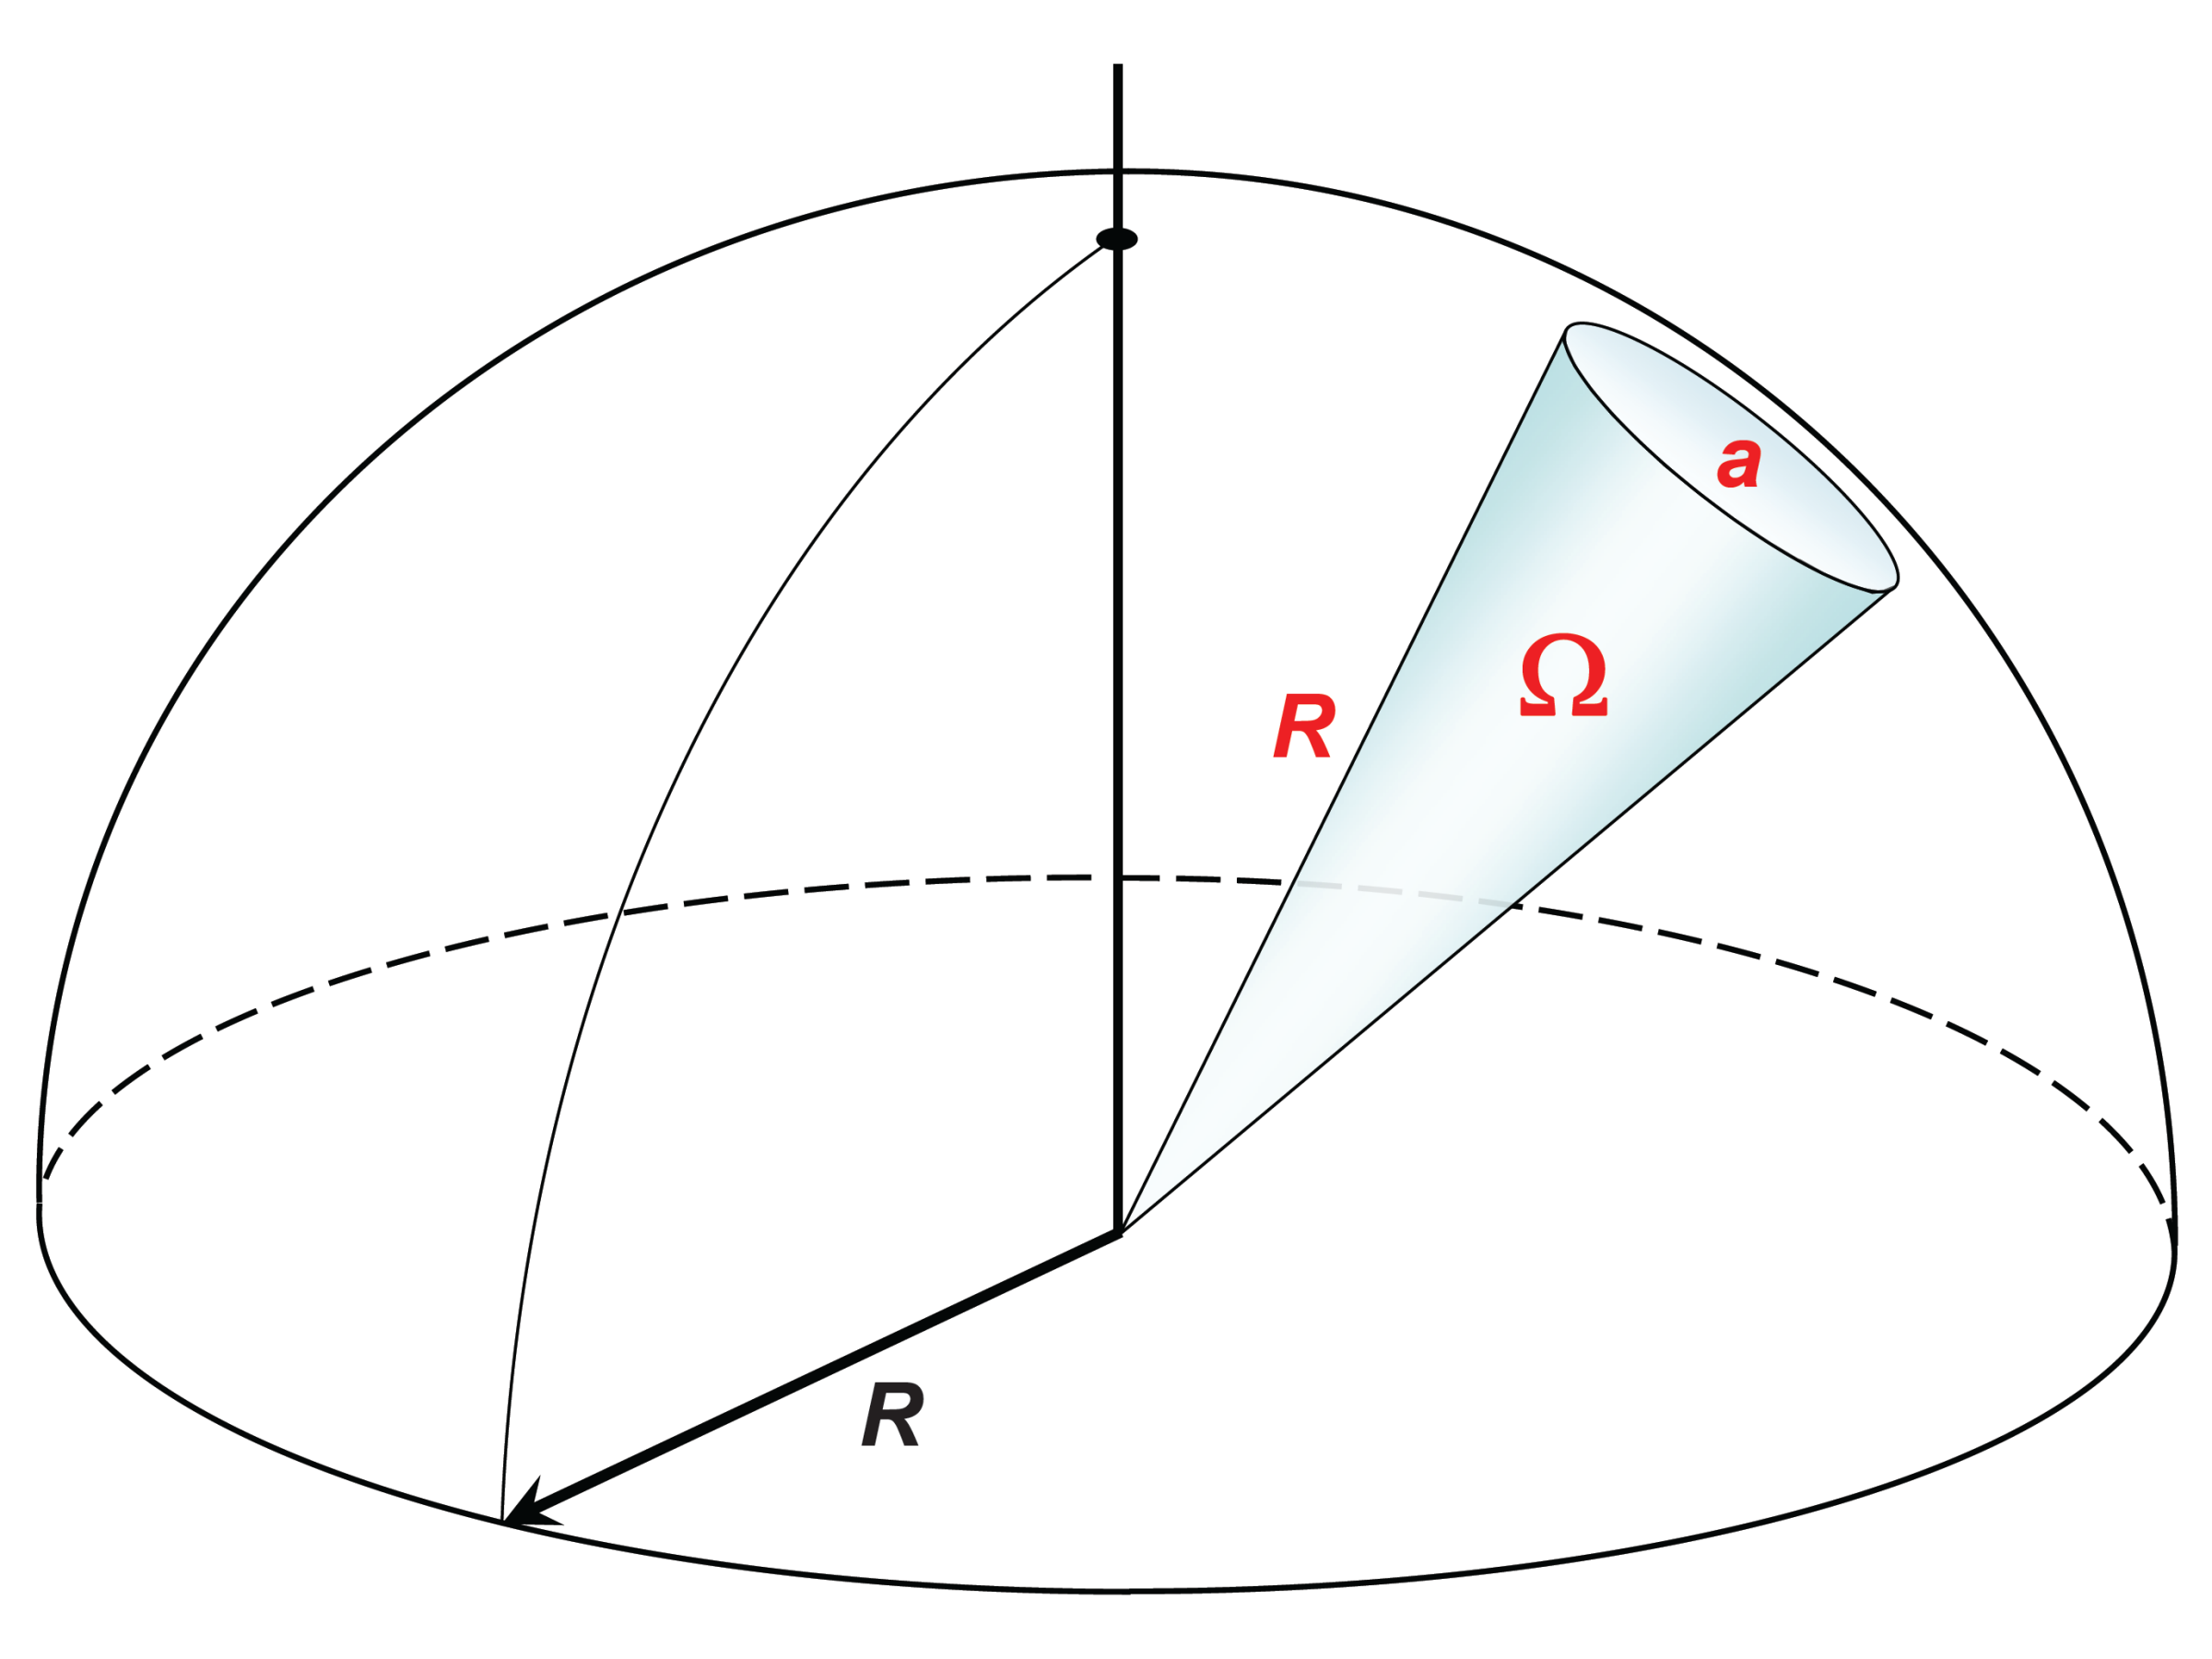
\includegraphics[scale=0.07]{images/solidangle.png}
%   \setcaptioncitation{https://socratic.org/questions/how-much-of-the-total-energy-that-leaves-the-sun-makes-it-to-earth-why}
  \caption{A depiction of the steradian, $\Omega$ of a conic surface area located on a sphere of radius $R$.}
  \label{solid_ang}
\end{figure}

We will get a steradian value for our setup by comparing angular separations to pixel distances in our camera images.
To expand on this, as the Moon travels through the night's sky, it changes locations on our observable hemisphere.
Differences in location on the hemisphere can be described by the angle they form with respect to the observer, the angular separation.
If it were to travel from one horizon directly through the zenith to the other horizon, it would have traveled an angular separation of $180 \deg$.  
If we know the angular separation traveled and the total number of pixels traversed, we can establish a relationship between the two and get a precise steradian value.
Plugging this value into Equation~\ref{area_eq} yields the area of sky observed.
Equation~\ref{area_eq} does well to describe a purely conic field of view.
As we will see see in our methods section, it is also useful to know the area of a rectangular pyramid.
Specifically, we want to know the surface area of a rectangular pyramid's base that has been projected to have a constant radius. 
This resulting area appears as a curved surface that could be imagined as a small square cutout of a sphere.
We see in Figure~\ref{useful_area_equation} a depiction of this shape as well as some equations that help calculate the base's surface area.
With respect to the two angles $a$ and $b$ that determine the size of the base, we find that:

\begin{equation}
\Omega =  4 \arcsin{(\sin{(\frac{a}{2})}\sin{(\frac{b}{2})})}
\label{steradian1}
\end{equation}

where $\Omega$ is the shape's steradian.  
The steradian can be further used to help find the area of the base via the formula:
\begin{equation}
\Omega = \frac{A}{r^2}
\label{steradian1}
\end{equation}
where $r$ represents the distance to the area of the sky you are observing.
Using basic substitution and algebra, we find that the resulting equation for the area of the base in terms of the distance $r$ and the two angles $a$ and $b$ is:

\begin{equation}
A =  4 \arcsin{(\sin{(\frac{a}{2})}\sin{(\frac{b}{2})})} r^2
\label{small_area_eq}
\end{equation}

where $r$ represents the distance to the area of the sky you are observing.
We will see this equation applied in the methods section when converting angular measurements to kilometer measurements.

One might naively assume that the total observation area would remain consistent each night.
However, one must consider clouds and fog when calculating the overall sky area coverage.
This consideration will be dealt with in our secondary analysis and is further discussed in the methods section.


\begin{figure}[ht!]
  \centering
  \includegraphics[scale=0.4]{images/rectangular_pyramid.png}
  \caption[A visual depiction of the surface area of the base of a fixed radius rectangular pyramid, marked $A$, alongside supporting equations.]{A visual depiction of the surface area of the base of a fixed radius rectangular pyramid, marked $A$, alongside supporting equations.  The steradian $\Omega$ is not marked on the leftmost figure because it represents an angle not visible and should not be confused with angles $a$ or $b$.}
  \label{useful_area_equation}
\end{figure}





\chapter{Methodology}

To calculate the flux of fireballs from our D6 AllSky Camera, we need to find the total observation area, time, and the total number of events.
In this section, we begin by describing in detail our methods for finding each of these properties.
Some time will be spend discussing obstacles such as camera fish-eye effect and cloud interference.  
Additionally, we will delve into the structure of our database: our fundamental tool for secondary statistical analysis.

\section{Calculating Total Observation Time}

Each night the D6 AllSky Camera observes, a program is run on the controlling Raspberry Pi that logs important information throughout the night.
The observation log is a simple time-stamped text file that records what processes the system runs at various times in a given night.
For instance, the observation log contains when each observation run begins (when the camera is set up initially), when the camera begins its analysis, when a new event is detected, and when the analysis goes to sleep, along with potential warnings or error messages that might come up.

To calculate the total observation time, we run a Python script that searches for the time associated with the start of each new analysis.  
After this time is recorded, we continue down the list of information until we find the time associated with that observation run's end.  
By subtracting the two times, we find the total observation time for that specific night.  
Performing this same method in a loop throughout all of the nights allows us to find how much time we spent observing on a given night. 
By summing up the total time observed over each night, we can attain the total observation time over the course of our data collection period.

A depiction of a portion of an observation log and our time analysis table can be seen in Figure~\ref{obslog_time}.
Note that while the information row that contains "New Observation Run Started" sounds as if it represents the start time, it does not.
A new observation run begins once the the D6 Camera is placed outside and turned on.  
Occasionally, the camera is set up while the sky is still too bright to begin actual video recordings. 
Therefore, we define our start time from a separate information row that states "A new night has arrived! Frame analysis beginning!". 
End times are determined by the information rows labeled "Day has come.  Analysis going to sleep."

\begin{figure}[ht!]
  \centering
  \includegraphics[scale=0.51]{images/obslog_time.png}
  \caption{An example observation log and the resulting time analysis information.}
  \label{obslog_time}
\end{figure}

Occasionally, we run tests on different D6 AllSky Camera actions. 
For example, we could program it to shut down, restart, or take pictures.
On August 29, 2018, one test resulted in no recorded "Day has come.  Analysis going to sleep." log.
This meant that we didn't have a correct log for that night's observation end time, leading to an error of a $14$ day observation session.
In actuality, the observation session was purely intended for testing and lasted less than one hour.  
Fringe cases like this raised red flags in our analysis and were looked at individually.
In all cases, these testing sessions were not considered part of our real observation.


It is imperative that we save not only the total observing time over a given night, but also the start and end times. 
This information is crucial for the next section, where we calculate the area of sky observed on a given night.

\section{Calculating Total Observation Area}

One of the most difficult problems we needed to address for this project was determining what area of the sky the D6 AllSky Camera observed each night.  
In an ideal world, our camera would be able to see all parts of the observable night sky, spanning across all horizons.  
However, due to optical limitations of our system and this is not possible.
Figure \ref{views_sidebyside} shows how our field of view is rectangular, as opposed to some other systems with a slightly more encompassing view.
This means that even if we new the total angular coverage of our camera with respect to the horizon, we wouldn't be able to precisely estimate our total observation area.
Nevertheless, determining the flux is a primary goal of this project, and is directly dependent on observation area. 

\begin{figure}[ht!]
  \makebox[\textwidth][c]{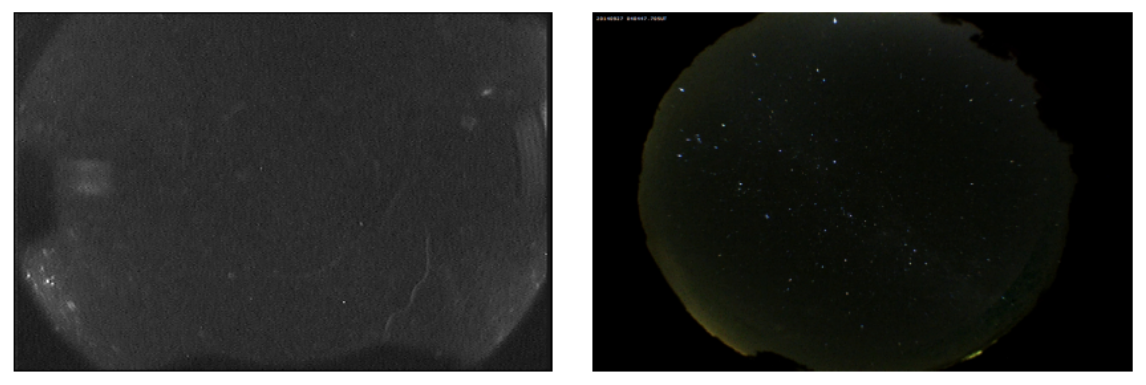
\includegraphics[width=1.0\textwidth]{images/allsky_view_sidebyside.png}}
  \caption{Left: our rectangular field of view.  Right:  A separate system's more complete circular view.}
  \label{views_sidebyside}
\end{figure}

To make matters more complicated, while the use of a fisheye lens gets us more coverage of the sky, it also results in some distortion of the image.
These distortions generally get worse the further an object is from is from zenith (directly overhead).
The significance of this problem as related to our project stems from the fact that while $50\% $ of our camera's pixels may be covered by clouds, this doesn't necessarily mean that $50\%$ of the observable sky is covered.
Therefore, we need some way of relating a given camera region to some observable distance.

To do this, we used observations of the Moon and various stars to calculate angular distance to pixel ratios for different regions of our camera.
This solution addresses the need to account for a camera fish-eye effect by assigning different fields-of-view to different pixel observational areas.
By correlating certain pixels with specific angular distances, we can analyze the available sky coverage by summing across all pixels.
To fully understand the methodology behind calculating the total observation area, one must understand how angular separation serves a role in area coverage.

\subsection{Angular Separation}

Consider two objects, both of which are visible to you, an observer.
One simple way to compare the two objects is by measuring the direct distance between them.
However, this isn't always known, especially when the objects are extremely far away.
An alternative way to compare the two would be to imagine two straight lines extending from your location to both objects.  
Because both lines are extending from the same location, we can calculate the associated angle between the two lines, known as the angular separation.
This angular separation may change as you move locations if the objects are nearby. However, if both objects are extremely far away, no small change in observer location will change the angular separation significantly.
We can essentially treat the two objects as points on a celestial sphere, with equal radial distance from the observer.  
Angles are a natural way of measuring displacement on a celestial sphere.


\begin{figure}[ht!]
  \centering
  \includegraphics[scale=0.53]{images/angdistances_explained.png}
  \caption{A theoretical depiction of two separate pixel regions' corresponding observable surface areas.  These areas are dependent on the angular coverage of that pixel region.}
  \label{angdist_exp}
\end{figure}


We can apply this concept and principle to calculate angular distances between stars and other celestial objects.
This intuitively makes sense because we don't necessarily know the extremely large distances to stars or between them.
We can therefore treat them like points on a celestial sphere and measure the angles between them.
Relating an angular distance to a pixel distance allows us to determine angular separation per pixel within that general pixel region.
By taking data on the angular and pixel separations between celestial objects across different pixel regions, we can estimate angular coverage in separate parts of our field of view independently.

We can eventually sum our findings across all pixel regions to calculate our camera's total angular coverage.  
Assuming that the fireballs are ablating in our atmosphere at a given height, we can then apply our angular measurements to attain an observational surface area as desired.
Figure \ref{angdist_exp} depicts a theoretical relationship between different pixel regions representing different angular areas.
We see that the surface area used in flux calculations is a slightly curved base of a rectangular pyramid, where the tip of that pyramid represents a pixel or pixel region.
Importantly,to calculate angular separation between many objects, we need to first have a database of objects to compare.

\subsection{Collecting a Star Catalog}

The D6 AllSky Camera not only captures video footage of fireballs, it also takes snapshots (pictures) throughout an observation night to aid in the larger fireball analysis vision.
The motivation behind this is primarily to check cloud coverage, but these images can store other important information.
Stars are visible in many D6 AllSky Camera's snapshots.  
The first step in creating a catalog of star information is recognizing stars within snapshots.  
We went about this by cleaning the image of hot spots, thresholding the image, and using the a \texttt{SimpleBlobDetector} to capture star locations.
All of these processes are coded and executed in Python.

\subsubsection{Hot Pixels and the Dark Frame}

Hot pixels are flawed pixels within a camera that always provide a significant positive photon count, even when the camera is exposed to complete darkness.
These pixels are problematic when trying to locate stars, as they don't represent any real physical object.
Fortunately, this source of error can be accounted for by taking an image while the lens of a camera is covered.  
This is called a dark frame, because the lens is not exposed to light.
Ideally the dark frame displays a black image, but most cameras will have a few hot pixels.
By subtracting this dark frame, represented by a 2-dimensional array of values ranging from $0$ to $255$, we are able to remove the hot pixel's effect from all other frames.
Figure \ref{hotpix} represents the an image, the dark frame, and that first image subtracted by the dark frame.



\begin{figure}[ht!]
  \makebox[\textwidth][c]{\includegraphics[width=1.0\textwidth]{images/og_darkframe_difference.png}}
  \caption{From left to right: an unaltered snapshot, the dark frame, and the dark frame subtracted from the original snapshot.  Note the region enclosed depicts a clear area of difference between the images.}
  \label{hotpix}
\end{figure}



\subsubsection{Thresholding}

Once these hot pixels are subtracted from a given frame of interest, the next step is to enact some type of threshold.
In this case, a threshold represents a cutoff photon brightness for every pixel.  
If a pixel has a count that is lower than the threshold, that photon count is changed to zero, which is pure black.  
Alternatively, if a pixel has a count that is higher, the  count becomes 255, or pure white.  

Thresholding serves the important role of simplifying an image to a purely black and white, on or off type image.
The necessary threshold for different images differed in accordance with the amount of surrounding light.
For the purposes of this project, we used an initial threshold of $140$.
If $140$ was not a sufficient threshold, this value was increased in increments of $5$ until the resulting image appeared to properly segment between open sky and clouds. 
For example, images that contained the Moon, a bright source that tends to wash out neighboring pixels, needed higher threshold values than images without.
Figure \ref{dif_thresholds} shows how different images may require different thresholds based on their original brightness.
The presence of clouds and/or the Moon also plays a significant role in this process.

\begin{figure}[ht!]
  \centering
  \includegraphics[scale=0.4]{images/different_thresholds.png}
  \caption{Two separate D6 snapshots alongside their thresholded images.  Note the differences in their respective threshold cutoff values.}
  \label{dif_thresholds}
\end{figure}

\subsubsection{SimpleBlobDetector and Stellarium}

Next, we use the \texttt{SimpleBlobDetector} function from the \texttt{CV2} library to detect potential stars.
This function is able to read an image and scan for objects that meet your specified parameters.
Variable parameters include, but are not limited to, size (in pixels), circularity, convexity, and color.
In this instance, the color filter has a value of $255$.
We filter based on area, scanning for stars between 1 and 20 pixels in size.
The star must lastly have a minimum circularity value of $0.5$.
When enacted, this function scans the picture and returns a list of detected locations where all of these parameters are met.
Using simple plotting functions, we can overlay these locations with the original image.

At this point, we have a list of potential object locations, but no foreseeable way of identifying the real ones.
As luck would have it, \textit{Stellarium}, a free astronomy software allows users to view a clear night sky from any point on Earth at any time.
Additionally, this interactive software stores information about the stars' names and other important information.
By viewing \textit{Stellarium} and a D6 AllSky snapshot and comparing the two, we are able to recognize which objects are real and which are false positives.
While hot pixels remove some false positives, random noise causes some pixels (or pixel groups) to resemble the size and color of stars.
Because each snapshot is labeled with the corresponding data and time, this method proved sufficient in identifying celestial objects from images.
A depiction of this process can be seen in Figure~\ref{star_recognition}.  
When comparing the two images, it should be clear that the objects numbered $17$, $16$, $19$, and $21$ correspond to Betelgeuse, Aldebaran, Capella, and Polaris. 
Also note that in the image, there are several recognized objects that don't have any celestial counterpart.
These are all false positives.
Similarly, there are cases in which the \texttt{SimpleBlobDetector} is not able to recognize an object that appears in a snapshot.

\begin{figure}[h]
  %\centering
  \makebox[\textwidth][c]{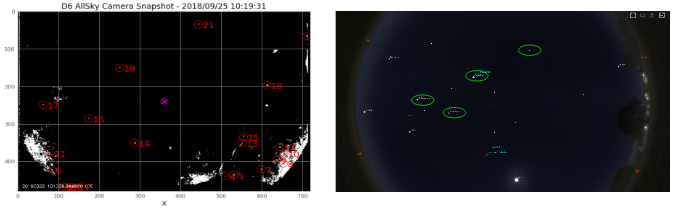
\includegraphics[width=1.0\textwidth]{images/stellarium_sidebyside.png}}
  %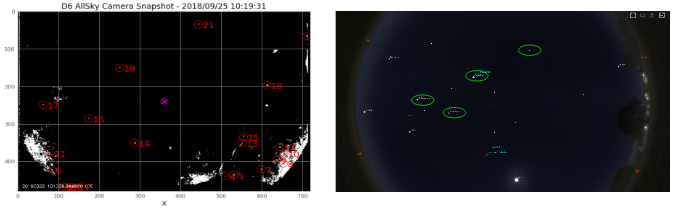
\includegraphics[scale=0.43]{images/stellarium_sidebyside.png}
  \caption{A D6 AllSky snapshot (left) alongside a Stellarium display (right).  We compare the two to find recognized stars that are found in both images.  These are circled in lime green in the Stellarium display. }
  \label{star_recognition}
\end{figure}


Once an object in a given frame is matched to a name, we used the Python library \texttt{Astroquery} and its function \texttt{Vizier} to automatically look up the star's right ascension, declination, V-magnitude, azimuth, and elevation.  
This, combined with the star's pixel location, time, and original snapshot's file name, was added to our star catalog as a singular data row.

\begin{figure}[h]
  \centering
  \includegraphics[scale=0.4]{images/az_el.png}
  \caption{A visualization of altitude and azimuth measurements on a unit sphere.  Note that a positive azimuth angular measurement moves from North towards East.}
  %   \setcaptioncitation{https://en.wikipedia.org/wiki/Horizontal_coordinate_system#/media/File:Azimuth-Altitude_schematic.svg}
  \label{altaz}
\end{figure}

\subsubsection{Azimuth and Elevation}

Each star has several inherent properties such as magnitude, right ascension, and declination.  
The later two represent coordinates that locate a star on the celestial sphere.  
Other properties, such as a star's azimuth and elevation change over time and vary dependent on the observers location.  
These two properties indicate a star's position in the sky relative to an observer and act similarly to spherical coordinates.

Figure \ref{altaz} shows how altitude and azimuth coordinates are determined. 
Note that the azimuth is an angle with respect to North.
A move closer to a pure East direction reflects a positive azimuth angle, whereas a move in the West direction reflects a negative azimuth angle.
Through finding the azimuth and elevation of a star, we can assign a star a 3-D coordinate value that lays on a unit sphere.  
We can then calculate the angular separation between two 3-D coordinates by taking advantage of properties of the dot product:

$$ \vec{A} \cdot \vec{B} = |\vec{A}||\vec{B}| \cos{(\theta)} $$

where $\theta$ represents the angular separation between the two unit vectors.  
Because we know that both vectors representing star locations will fall on a unit sphere, their magnitude is $1$.
Using this knowledge, we may transform the above equation to:

$$ \theta = \arccos{(\vec{A} \cdot \vec{B})} $$

Given this formula we calculate the angular distance that separates two different celestial objects.
The average angular distance per pixel measurement is determined by taking the angular distance divided by the pixel distance between the two celestial objects' pixel locations.
This equation is important and can be seen the following equation:

$$ \textrm{Avg. Angular Distance per Pixel} = \frac{\theta}{\textrm{pixel separation}} $$




\subsection{Calculating Angular Areas}

The D6 AllSky Camera is a versatile system and it's orientation and position can change slightly from night to night.
Because of this, there are several considerations that must be accounted for when calculating angular distance per pixel across different camera regions.
The D6 AllSky Camera is a versatile observation tool, and it therefore takes observations in slightly different locations each time it is put out.
A change in observation location could mean that if one night a star is located at pixel value $(10,10)$, and the next night it could be located at $(94,134)$.
We have developed a method for calculating angular separation per pixel data points that account for this consideration.

\subsubsection{Comparing Objects from the same Night}

The star catalog stores information about celestial objects over the course of all observations.
Using constraints from the Time Analysis information (start time, end time, time elapsed), we can isolate rows within the star catalog from a specific night.  
After creating this subsection, we can then use our described method to calculate the angular separation per pixel for every combination of two objects.
One might question where the data behind this angular distance per pixel should be located.
After all, there are two different object locations used to calculate the value.
Our strategy was to locate the point in between the two objects.  
Figure~\ref{starcombos} depicts these combinations along with the locations of the angular separation per pixel represented as white dots.

\begin{figure}[ht!]
  \centering
  \includegraphics[scale=0.70]{images/star_combinations.png}
  \caption{A set of four stars (yellow) that could be compared to calculate six separate angular distance per pixel data points (white).}
  \label{starcombos}
\end{figure}

Figure~\ref{starcombos} gives a general depiction of our method on a much smaller scale.
Note that when comparing objects from this subsection of the star catalog, we are not limited to only comparing different stars.
As an object moves throughout the night sky, its azimuth and elevation change along with its pixel location.
We can thus treat each individual observation as a unique object, even comparing between the same object at different times throughout the night.
This creates many more combinations than if we were to only consider unique stars.

After calculating all potential angular separation per pixel values alongside their location information, we may move on to calculating average angular separation per pixel in different camera regions.
For the sake of dividing our field of view into different pixel regions, we split up our $720 \times 480$ pixel camera frame into $40 \times 40$ pixel squares.
This also allows us to observe the difference in angular distance per pixel ratios across the entire field of view

\begin{figure}[h]
  \centering
  \makebox[\textwidth][c]{\includegraphics[width=1.0\textwidth]{images/rotated_pixels.png}}
  \caption{Left: our angular separation per pixel data set. Right: that same data set with two rotated and appended data sets.}
  \label{rotate}
\end{figure}


There are $216$ total pixel regions and only so many angular separation per pixel data points.
Some pixel regions that do not contain any data points.
By assuming that our field of view has rotational symmetry, we can rotate and append new data to our set.
Figure \ref{rotate} shows one data set that is rotated twice in $10 \degree$ increments.
For the sake of this project, we rotated our original data $360 \degree$ in $5 \degree$.  
This allowed us to fill in all of the empty regions and multiply our data set quantity by over $50$.
All angular separation per pixel measurements located inside a given square were then averaged over to determine that square's average angular separation per pixel value.

\section{Calculating Cloud Coverage}

The D6 AllSky Camera currently does not always remain outside.
For the most part, our camera was only placed outside during nights where observation conditions were promising.
Because we cannot see or properly analyze fireball events that happen behind clouds, we cannot count cloudy regions as observable areas.
As mentioned previously, the D6 AllSky Camera takes several snapshots of the night sky systematically throughout an observing session.
Specifically, it currently takes images every $30$ minutes.
By using thresholding, we have seen how we can determine which pixels qualify as not observable areas.
The threshold value that we used in this step was a photon value of $90$.


We chose a different threshold pixel value for this cloud analysis than the threshold in our star recognition program.
While thresholding for star recognition, we want to minimize the number of false positives.
The more distinguishable bright small objects in a given frame, (ex: pixels on the edge of a cloud) the larger number of objects that meet our \texttt{SimpleBlobDetector} parameters.
This adds a hefty bulk of time sifting through false positive objects.
While trying to find clouds, we don't want to get rid of hazy cloud boundaries, so we utilize a lower threshold.

Unfortunately, some pixels that fall within a broad cloud area are not recognized through this process.
The solution to this problem lies in the \texttt{OpenCV} functions \texttt{MORPH\_CLOSE} and \texttt{MORPH\_ERODE}.
The first of these functions fills in regions of empty space that are next to filled in space.
This is helpful in closing gaps between pixels that represent clouds.
However, because the edges of the clouds are expanded in this process, we must subsequently perform a \texttt{MORPH\_ERODE} that works in the opposite fashion.
Once a hole is completely closed, there is no space within a cloud for the eroding function to open up, hence providing a satisfying answer to the cloud predicament. 
The difference between a thresholded image and the subsequently closed/eroded image can be seen in the upper-right and lower-left panels of Fig. ~\ref{colorclouds}.
We may observe that this method fills in a vast majority of the small dark holes in the thresholded image.

After this successful threshold and subsequent closing/eroding process is complete, the next step is implementing the relationships between pixels and angular distance.
By assigning the correct regional angular separation per pixel value to each pixel within a cloud, we are able to estimate the angular area that cloud covers.
Figure~\ref{colorclouds} shows the processes taken in calculating the area occupied by clouds.
Note that both a filling and eroding function was used to attain the lower left image.
The observable area during that time is the cloud coverage subtracted from the total observation area.


\begin{figure}[ht!]
  \centering
  \includegraphics[scale=0.4]{images/Cloud_analysis.png}
  \caption[Calculating cloud area coverage from thresholding and applying our angular distance per pixel map.]{From top left to bottom right: a cloudy D6 snapshot, that snapshot with a threshold applied, the thresholded image after a close/erode function was applied, the subsequent pixels assigned angular distance per pixel measurements.  The angular distance per pixel map is discussed more thoroughly in the Data chapter.}
  \label{colorclouds}
\end{figure}

This process is performed for each snapshot.
In creating our average area observed calculations, we assume that the sky retains that same amount of cloud coverage for the $15$ minutes prior to and $15$ minutes after the snapshot.
While this isn't precise down to the exact minute, over many observations, the number of over-estimations and under-estimations should average out and yield an accurate observational area.























 

\chapter{Data}

Because there is intrinsic variability in the number of near-Earth objects colliding with Earth's atmosphere from night to night, a sufficiently large data sample plays a vital role in estimating an average flux.
This chapter details our data sample.
Specifically we will discuss into observable time, observable area, and number of events.  
To assess the overall capabilities of our system, we also delve into the data behind our star catalog, previously used for total observable area calculations.  
This chapter provides the raw data and overall distribution and shape of the data. Further analysis and interpretation of the data can be found in Chapter 5.

\section{Time Distributions}

While the D6 AllSky Camera has a protective watertight shell, it is currently not always placed outside for nightly observations due to precaution and convenience.
Due to Oregon's climate, we often leave our observation system inside.
There have been a total of $221$ days between August 27, 2018, the beginning of Willamette's academic year, and May 6, 2019.
Out of those $221$ days, we have observed during $34$ nights, for a total of $291.87$ hours.

When outside, the D6 AllSky Camera automatically begins observation runs when the sky is dark enough to take videos of without fear of over-saturation.
As the sky gets brighter when sunrise approaches, the camera automatically shuts off, ending the observation session.
This brightness constraint means that the total observation time changes from night to night.
During observation nights, we observed for an average of $8.584$ hours per night.
The shortest observation session lasted $7$ hours while the longest lasted $11$ hours.

Figure~\ref{dateplot} displays the individual nights that we observed throughout the academic calendar. 
In addition to plotting our observation dates and each session's total observing time, we have indicated dates of meteor showers visible in Salem, Oregon.  
During the months of October and November, we observed on nights of the Orionid and Leonid showers respectively.  
% Insert smooth transition

\begin{figure}[ht!]
  \centering
  \includegraphics[scale=0.25]{images/nights_observed_with_meteorshowers.png}
  \caption[A plot of all D6 AllSky observation dates and recognized meteor showers within the $2018-2019$ academic calendar year.]{A plot of all D6 AllSky observation dates and recognized meteor showers within the $2018-2019$ academic calendar year.  Note significant time gaps between observations as well as crossover between observations and meteor showers.}
  \label{dateplot}
\end{figure}




\section{Coverage Distributions}

As described in the methodology section, to calculate the angular distance per pixel for a given location, we needed two celestial object measurements.
These measurements can represent data from the same objects, but the two must have different pixel locations.
By taking the angular separation between the two, we designated the ratio to be at the midpoint between both locations.  
In total, we used $3279$ different comparisons to compile our angular distance per pixel dataset.  
Figure~\ref{angperpix1} shows all of these points, each colored with their respective angular separation per pixel ratio. 
We observe that some data points seem to follow natural arcs.
This is a result of to same-celestial object comparisons as they arc through the night's sky over time.


\begin{figure}[ht!]
  \centering
  \includegraphics[scale=0.47]{images/angular_distance_at_various_locations.png}
  \caption[A plot of initial angular distance per pixel measurements from celestial comparisons before rotation.]{A plot of initial angular distance per pixel measurements from celestial comparisons before rotation.  Here we see that a radial symmetry argument is necessary to get data points in bins that are not covered.  The arc-like patter in the data is representative of the path of a celestial object through the night's sky.}
  \label{angperpix1}
\end{figure}

One may note that Figure~\ref{angperpix1} shows many data points, but they do not span the entirety of the camera field. 
By rotating our initial data and appending it to a larger data set in sequences of $5\degree$ in a full unit circle, we were able to increase the number of data points by a magnitude of $71.22$ and cover all pixel regions in our field of view.
From this point we were able to then bin the data and create Fig~\ref{colorful}.
We bin and average the data to get an overall idea of how pixel distances relate to angular distances in different smaller regions.
Fig~\ref{colorful} shows how these average relationships vary in different regions of our field of view, as indicated by their color value.

\begin{figure}[ht!]
  \centering
  \includegraphics[scale=0.35]{images/boxes_colored.png}
  \caption[Average angular separation per pixel for different camera pixel regions.]{Average angular separation per pixel for different camera pixel regions.  We observe a larger angular separation per pixel closer to the horizon.  This aligns well with our prediction of the fish-eye camera's effect. Note the color bar reads differently than the previous image.}
  \label{colorful}
\end{figure}

As described in the Background chapter, we used our measured solid angles for each region to calculate individual  curved-rectangular areas at a fixed radius of \SI{11.4}{\kilo\meter}.
Our measured total areal coverage was  \SI{48363.33}{\square\kilo\meter}.

As some nights were cloudy and others clear, the observable area fluctuated from night to night. 
Figure~\ref{time_area} summarizes the total observation time and the average observable area for each of our observation months. 

\begin{figure}[ht!]
  \centering
  \makebox[\textwidth][c]{\includegraphics[width=1.0\textwidth]{images/time_vs_areaobs_plot.png}}
  \caption[A plot of total observation time and average observable area for each month.]{A plot of total observation time and average observable area for each month.  Note that in October we observed for the longest and under the worst observable area conditions.  This is likely a result of the two meteor showers that occur during that month.  We see a dip in time observed as we approach winter/early spring months, as expected.}
  \label{time_area}
\end{figure}

Our average observable area across all observations was  \SI{46178.81}{\square\kilo\meter}.
This value, along with our total observation time and number of events was used to determine the overall average flux.

\section{Detected Fireballs}

In total, the D6 AllSky Camera captured a total of $1077$ videos.  
Of those $1077$, only $6$ were identified as real fireballs.
Most of these false positives were caused by fast moving clouds or bugs.
In November, we began running a newly implemented secondary analysis that was created by Jed Rembold.
This analysis greatly reduces the number of false positives.
In the three months prior to the implementation of this analysis, there were $793$ videos from $3$ months of data.
Post-implementation, we captured $284$ videos in the remaining $4$ months containing observations.
A depiction of the locations of our captured fireballs is shown in Figure~\ref{fireball_locs}.
While the data sample is still small, we can observe that the locations of these fireballs are not dependent on a specific region of our field of view.  

\begin{figure}[ht!]
  \centering
  \includegraphics[scale=0.25]{images/fireball_initlocs.png}
  \caption[The initial pixel locations of all detected fireballs with respect to our field of view.]{The initial pixel locations of all detected fireballs with respect to our field of view.  Note that the locations are not dependent or specific to any region in our field of view.}
  \label{fireball_locs}
\end{figure}

Of the $6$ fireballs, $3$ were found within $24$ hours of the Leonid meteor shower while $1$ more was found during the Orionid meteor shower.  

Unfortunately, the photometry program used to analyze fireball light-curves had issues processing each of these cases, and there was not enough time to troubleshoot and fix that program.  
Therefore, we do not have calibrated luminosities for our observed fireballs and can not make a prediction of their energy or mass at the moment. 


\section{Camera Capabilities}

As described in Chapter 3, the star catalog consists of recognized stars from the D6 AllSky Camera's snapshots.
In a catalog containing a total of $387$ celestial object observations we observed an average of $1.44$ stars per snapshot containing at least one star.
In total, the system took $1638$ snapshots or videos that could be condensed to snapshots via frame-stacking.
$269$ of these contained identifiable celestial objects (stars or the Moon).  
Within our star catalog, we captured information on $14$ unique objects.
Of these objects, the dimmest, Alpheratz, had a visible apparent magnitude of $2$. 
Sirius was our brightest recognized star, having a magnitude of $-1.46$.
It should be noted that the Moon, having an apparent magnitude of $-12.74$, is significantly brighter than any observable star apart from the sun.


\section{Flux}

After attaining the number of events, total observation time, and average observational area, we found that the D6 AllSky Camera had an average flux of \SI{4.45E-7}{\per\hour\per\square\kilo\meter}.
Table~\ref{table1} displays this value alongside the values that contributed to our flux calculation. 
As a point of comparison, Dr.~Jed Rembold measured an average flux rate of \SI{1.09E-7}{\per\hour\per\square\kilo\meter} when studying meteor impacts on the Moon \cite{jed_dissertation_2014}. 
Clearly the Moon and Earth are inherently two different objects with different gravitational effects.
However they have similar locations within our solar system, and thus their average flux rates should share some resemblance.
The fact that the D6 AllSky Camera's fireball flux rate shares the same order of magnitude as other meteor research is promising.  
While we can't make any definitive claims about the feasibility of our camera system, we remain cautiously optimistic. 



\begin{table}[ht]
\setlength\extrarowheight{5pt}
\centering
\begin{tabular}{lll}
\toprule
& D6 AllSky Camera & Lunar Impacts \\
\midrule
Number of Events & $6$ & $51$  \\
%\hline
Average Area (km$^2$) & $46,178.81$ & $5.77 \times 10^{6}$ \\
%\hline
Total Time (hr) & $291.87$ & $80.97$ \\
\midrule
Flux (hr$^{-1}$km$^{-2}$) & $4.45 \times 10^{-7}$ & $(1.09 \pm 0.02) \times 10^{-7}$ \\
\bottomrule
%\hline
\end{tabular}
\caption[A display of our average flux rate alongside contributing variables compared to lunar impact flux rates measured by Dr. Jed Rembold \cite{jed_dissertation_2014}.]{A display of our average flux rate alongside contributing variables compared to lunar impact flux rates measured by Dr. Jed Rembold \cite{jed_dissertation_2014}. Note that while the many of the contributing variables are significantly different, both flux measurements are on the same order of magnitude.}
\label{table1}
\end{table}



\chapter{Conclusion}

Calculating average flux only depends on three variables. 
Although this calculation appears simple, estimating an average observational area can extremely difficult. 
Through establishing a method for calculating observable sky area that works for variable cloud coverage, we can now estimate the D6 AllSky Camera's average flux and compare it to other systems.
As of this point, our data sample is too small to make any conclusive claims.  
As such, there are still steps that need to be taken to truly assess the feasibility of using the D6 AllSky Camera in fireball research.
This section will detail some of our self-assessed points of critique as well as shed light on some possible future research directions.


\section{Critique}

While there are a multitude of positives to take away from this research, there are many areas of improvement as well.  
The main critique of our work stems from a lack of sufficient data.
Flux estimates rely on a robust data sample, something that we were not able to attain this academic year. 
In the Fall of 2018, we also experienced some camera noise difficulties that provided complications for our photometric analysis.


\subsection{Data Size}

Throughout the history of fireball research, a sufficient data size has proven to be a vital characteristic of most notable findings.
In 1996, the Canadian camera network published a detailed analysis of the $259$ fireballs captured by their system \cite{halliday_innisfree_1981}.
Peter Brown, one of the most recognized figures in fireball research, released a paper in 2002 that detailed an analysis of $300$ fireballs as captured by the departments of Energy and Defense. \cite{brown_p_flux_2002}.
Surveys like these two have the luxury of calculating detailed flux estimates for fireballs with different energies or masses.
This is mostly due to their large data samples and aided by low-error margins that they get from extremely precise instruments.
By binning fireballs that share similar properties, these research groups can measure relationships between likelyhood of impact and fireball properties.
The value of average flux is often replaced then by the more detailed fireball energy distribution.
This makes comparing our system to existing systems slightly more difficult since net fireball flux rates are not always so widely reported.


Our system has captured a small fraction of the total number of events found in the aforementioned research papers.
Our lack of data isn't necessarily due to a lack of camera capability, and likely has to do with the total time observed. 
Observing a total of $34$ nights out of a possible $221$ yields a ratio of observing a little less than $16\%$ of nights. 
This low ratio is partially due to poor weather.
However, there were also nights where the camera was not placed outside due to scheduling complications.
As we gain more confidence in our camera system's capabilities, we will begin to leave the camera in the field to observe for longer chunks of time to avoid such complications.
Observing for more nights and capturing a larger number of fireball events will allow for more points of comparison to existing surveys.
This will in turn allow us to gain a stronger understanding of how our camera system compares to current professional systems.


\subsection{Camera Difficulties}

In the early spring of 2019, the D6 AllSky Camera began having difficulty focusing on the night sky.
This led to images and videos containing lots of systematic noise.  
Figure~\ref{camera_noise} depicts the difference between an image with low and high noise.
Both images were taken with our same camera.
From these two images, it is clear that images and videos with high noise are more difficult to analyze.
Because we rely entirely on pixel photon counts for fireball property calculations, having clean images with minimal noise is imperative.
While we believe that it is not the primary cause, noise could be one factor contributing to our Photometry GUI's incompatibility with current data.
The main issue stems from a fireball-tracking program that needs some slight tweaking.

\begin{figure}[ht!]
  \centering
    \makebox[\textwidth][c]{\includegraphics[width=1.2\textwidth]{images/low_and_high_noise.png}}
  \caption[A low noise D6 snapshot taken in August 2018 (left) alongside a high noise D6 snapshot taken in December 2018 (right).]{A low noise D6 snapshot taken in August 2018 (left) alongside a high noise D6 snapshot taken in December 2018 (right).  Noisy pixels provide issues for photometric analysis, which serves the foundation for fireball property estimates.}  
  \label{camera_noise}
\end{figure}

Not only was the camera noise problematic for photometric analysis, but it also made star recognition more difficult.
In many D6 snapshots, we were unable to recognize any celestial objects.
A lower-noise level could allow us to recognize more stars which would add to our star catalog, and increase the number of data points used to determine observable area.
There is also a chance that we could detect dimmer stars with less-noisy data, leading to a stronger understanding of our camera's capabilities.

\section{Outlook}

Moving forward, the most important thing to focus on is data collection.
Once the problem with unusually high volumes of systematic noise is dealt with, we will have most of the framework established to create a running fireball catalog.
However, we will need to create a script that estimates a fireball's properties (energy, mass, size) given the photometry program's outputted light curve.
This project however should be fairly straightforward and will utilize the equations such as Eq. \ref{area_eq} in the background chapter.

While a singular camera can serve an important role in fireball research, systems with multiple cameras stationed in different locations have certain benefits.
They allow for the triangulation of a given fireball which can then lead to more accurate velocity and position estimates.
With multiple systems, we could also estimate a fireball's orbital elements, and thus determine from whence it originated.
If we come to the conclusion that the D6 AllSky Camera is a feasible alternative in fireball research, we hope to construct another D6 AllSky Camera that will lead to more precise data collection. 
The prospect of a secondary system is exciting and will hopefully help prove that the D6 AllSky camera is a desirable alternative in fireball research.
%\input{appendix.tex}

%\bibliographystyle{urcsbiblio}
%\bibliographystyle{amsalpha}
%\bibliography{thesis_bib}
\printbibliography

%\appendix
%\include{notebook}

\end{document}
